\chapter{Digital pathology}
\label{chap:backdp}

\begin{overview}{Overview}
  The goal of this chapter is to provide digital pathology background  and keys to understand our contributions. We will focus our attention on topics relevant to this thesis. 
  
  Section \ref{sec:backdp:whatisdp} introduces and defines medical terms such as \textit{pathology}, defines \acrfirstit{dp} and introduces the notion of \acrfirstit{wsi}. Section \ref{sec:backdp:wsi} presents the journey of a sample from the body to the \acrshort{wsi}, introducing the different sources of variability introduced by the whole conversion process. 
\end{overview}

% analogintelligence.com image dp illustration

\section{What is digital pathology?}
\label{sec:backdp:whatisdp}

Nowadays, medicine and healthcare rely heavily on analysis of human body samples to study and diagnose diseases. The branch of medicine focusing on this analysis is called \textit{pathology} which includes histology-based pathology (\aka histopathology) and cytology-based pathology (\aka cytopathology). Both of these sub-branches involve the study of microscope glass slides containing samples (see Figure \ref{fig:backdp:glassslides}). In the case of histology, these samples are tissue sections cut from a bodily specimen. Cytology, on the other hand, is concerned with samples of free cells or tissue fragments which can be extracted by different techniques. 

\begin{figure}
  \centering
  \subfloat[Glass slide]{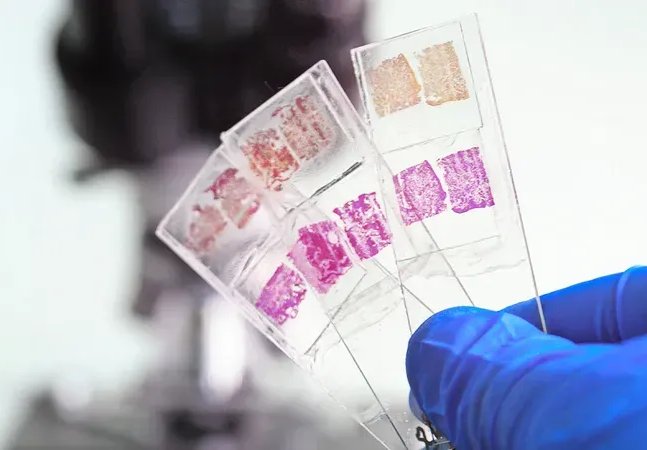
\includegraphics[scale=0.35]{backdp/microscope-slide.png}}\quad
  \subfloat[Whole-slide image]{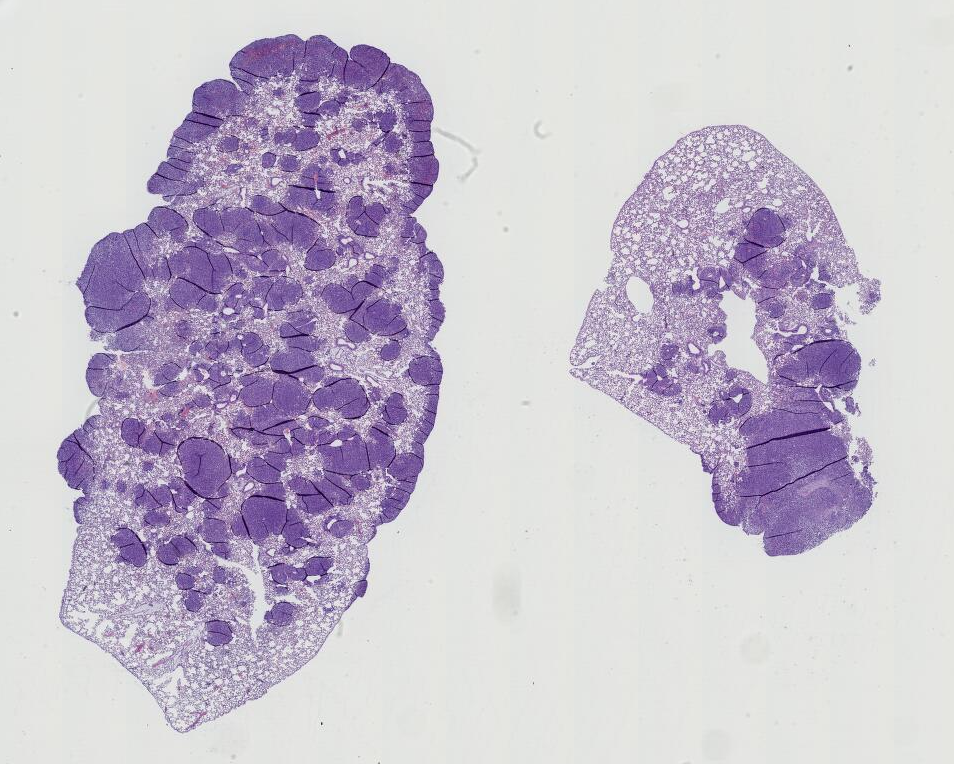
\includegraphics[scale=0.22]{backdp/wsi.png}}
  \caption{Microscope slides with tissue samples (images from \parencite{img:glassslides} and \TODO{reference demo cytomine}).}
  \label{fig:backdp:glassslides}
\end{figure}

The trend of digitalization affecting our societies also impacts pathology as, using dedicated scanners, these glass slides can now be digitized into large image files called \acrfirstit{wsi}. In this context, \acrfirstit{dp} can be defined as ``\textit{the acquisition, management, sharing and interpretation of pathology information — including slides and data — in a digital environment}'' \parencite{doolan2019whatisdp}. Working with \acrshort{wsi} instead of physical slides has several advantages and drawbacks (see Table 1 in \parencite{jahn2020digital} for a thorough list). Aside from easier sharing and storing of slides, digitization also opens the way for automated analysis sofware to automatically extract relevant information. Such software have the potential to relieve pathologists from time-consuming tasks allowing them to focus on challenging cases and research therefore reducing healthcare cost and improving diagnosis quality. According to the 2020 report on cancer from \acrfirstit{who} \parencite{world2020report}, the ratio of pathologist per inhabitant was approximately 1 per 15000 in high income countries but dramatically dropping to 1 er 1 million or less many low income countries. AI-assisted pathology therefore holds even greater promises for coverage and quality of healthcare in these countries where pathologists are rare.

Interestingly, although digitization technologies are quite mature, adoption of \acrlong{dp} in healthcare facilities is not simple. Many still heavily rely on glass slides for day-to-day operations. Indeed, the transformation requires significant investments (both in time and money) and careful planning to carry it out successfully which is not always comptabile with the workload of pathology services. Experienced pathologists are sometimes reluctant to change and lack confidence in modern tools for slide visualization and analysis. Moreover, some tasks cannot be performed easily on \acrlong{wsi}s but can on a glass slide (\eg exploring the depth of a sample in cytology by changing the focal plane). 

As far as automated analysis is concerned, it remains quite a challenge. Whole-slide images typically contain several gigapixels and cannot be loaded entirely in a typical computer memory at full resolution. Moreover, for most tasks, the image content is complex and classical computer vision methods would often fail to distinguish structures of interest. This complexity is due in particular to the presence of artifacts \parencite{taqi2018review} appearing during the conversion process of a bodily specimen to an image (see Section \ref{sec:backdp:wsi}). The ability of learning techniques to train models that capture complex relationships in data makes machine learning an ideal candidate to tackle \acrlong{dp} tasks. However, data scarcity is a prevalent issue in the field as quality data, especially annotated, can be difficult to obtain for various reasons: privacy concerns, time-consuming and expensive nature of the annotation process, \etc.     

Overall, digital pathology holds great promises but presents significant and interesting challenges on several fronts. This thesis focuses on the \acrshort{ml}-based automated analysis aspects of digital pathology and studies how to tackle data scarcity.

\section{Whole-slide images: a journey from the body to the computer}
\label{sec:backdp:wsi}

Turning a bodily specimen into \acrlong{wsi}s is a long and complex multi-step process typically involving the work of several highly-specialized technicians. Some steps can nowadays be automated but the chain remains mostly manual. In this section, we describe the different steps of this procedure (see \parencite{mccann2014automated} for an alternate and more detailed presentation with illustrations). With each step of the procedure comes the risk of introducing artifacts of which we will provide few examples. For a more complete list of pre-scan artifacts with illustrations, see \parencite{taqi2018review}. 

\TODO{talk about how this process can change for different type of samples => cytology???}

\subsection{Samples collection, fixation, cutting and dehydratation}

Whereas we focus mostly on histo- and cyto-pathology in this thesis, a pathology service typically deals with more than these two modalities. The specimens they receive for analysis range from small (commonly referred to as \textit{biopsies}) to very large (whole organ or body). Whole bodies are usually destined for autopsies which might themselves generate biopsies. Smaller speciemens (organs, biopsies) must be fixated before going through the next steps. 

The goal of fixation is to put a stop to the natural decay of the specimen and increase its structural stability \parencite{rolls2012process}. This can be achieved, for instance, by immersing the specimen in a formaldehyde bath (\ie the fixative solution) for period of time depending on its size (\ie few hours to a whole day). 

When the specimen has been fixated, it is then placed into a standardized container called a \textit{cassette} (see Figure \ref{fig:backdp:cassette}). If the sample is too large for the cassette, a volume of interest is cut from the specimen. Depending on the later examination, the orientation of the cut can be crucial to exhibit relevant tissue structures of the specimen. In the remaininder, we will call a \textit{sample} the content of this cassette.

For a proper analysis, the cellular morphology of the sample must be preserved. This is most commonly achieved by infiltrating the tissue with paraffin wax. Infiltration however does not work on a raw fixated tissue because paraffin is hydrophobic. Therefore, one must first perform \textit{dehydratation}, that is, to replace water naturally present in the sample with a product miscible with parrafin. This is done by first plunging the sample into a succession of alcoholic solutions baths. Although this process achieve dehydratation, alcohol does not mix with paraffin neither. Therefore, the sample is then plunged into one or more xylene-based solutions baths, xylene being miscible with both alcohol and paraffin. The sample, infiltrated with xylene, is finally plunged in a paraffin bath under vacuum \TODO{how does it work the vaccum stuff???}. The dehydratation process takes few hours and is often automated using dedicated machines.  

Artifacts can appear as early as at extraction of the specimen and even before. Each of the specimen and sample processing steps presented in this section can also introduce artifacts. Tissue can be damaged at specimen extraction site by the use of medical tools or treatment. Bad fixation can lead to decaying tissue (\ie autolysis) and structural degradation (\eg tissue shrinkage). Improper cutting can also cause tissue damage like tearing, squeezing and burning. Dehydratation has also its own set of possible artifacts. Improper dehydratation can leave some parts of the sample with remaining water, alcholol or xylene which. Tissues can also be exposed to the different solutions for an excessive duration. These processing errors can for instance cause tearing, shrinkage, interference with the staining process (see Section \ref{ssec:backdp:staining}) and affect the structural properties of the tissue (\eg the tissue becomes brittle). Automation obviously reduces the risk of mistakes and artifacts.

\TODO{big figure illustrating ``all'' possible artifactsand variations}

\begin{figure}
  \centering
  \subfloat[This is an example of well-fixed tissue showing good nuclear and cytoplasmic morphology with minimal shrinkage showing clearly defined basement membranes and cell margins.]{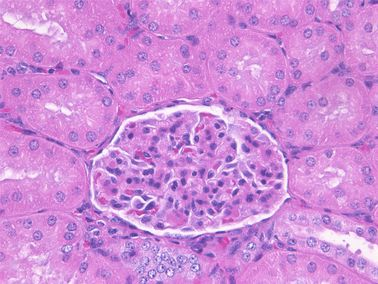
\includegraphics[scale=1.0]{backdp/fixationgood.png}\label{fig:backdp:goodfixation}}\quad
  
  \subfloat[This is an example of poorly-fixed tissue showing inferior nuclear and cytoplasmic morphology with excessive shrinkage and poorly defined cell margins.]{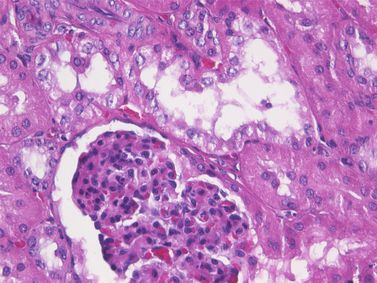
\includegraphics[scale=1.0]{backdp/fixationbad.jpg}\label{fig:backdp:badfixation}}
    
  \caption{Examples of good and bad fixations (images and sub-captions from \parencite{rolls2012process}).}
  \label{fig:backdp:fixation}
\end{figure}

\begin{figure}
  \centering
  \subfloat[Cassette with fixated samples (image \\ from \parencite{stidworthy2011getting})]{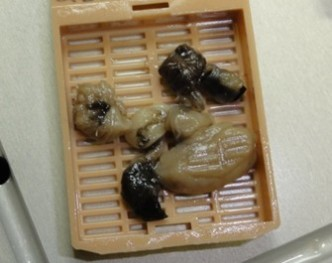
\includegraphics[scale=0.75]{backdp/cassette.jpg}\label{fig:backdp:cassette}}\quad
  \subfloat[Cassette with parrafin-embedded \\ samples (image from \parencite{img:cassetteparrafin})]{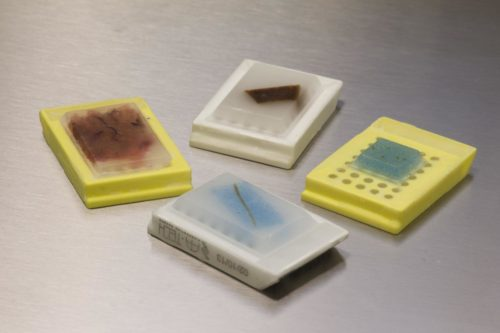
\includegraphics[scale=0.42]{backdp/cassette-parrafin.jpg}\label{fig:backdp:cassette-parrafin}}
  \caption{Tissue cassettes.}
\end{figure}

\subsection{Embedding, microtomy and glass-slide application}
\label{ssec:backdp:embedding}

At this point, the sample in the cassette has been infiltrated with paraffin. The next step consists in embedding the infiltrated sample in a block of paraffin to allow easier cutting. The sample is placed in a small container attached to the back of the cassette. This container will serve as a mold for casting the block of parrafin (see Figure \ref{fig:backdp:cassette-parrafin}). The block casting and hardening process takes When the block has solidified, the sample can now be cut into thin slices to be applied on the glass slides. Cuting is performed with a dedicated tool called a \textit{microtome} (see Figure \TODO{illus microtome}). Operated by a technician, the microtome allows slices to be cut to an extremely small and precise thickness of around 3 or 4 $\mu m$. The cutted slices are then floated onto a water bath which helps mouting them on glass-slides. 

These steps should be performed carefully not to introduce artifacts. For instance, a warm parrafin block or a dull microtome blade can cause compression artifacts (\ie tissue displacement causing material accumulation). Another possible source of artifact is contamination of the water bath with previous samples, hair, dust which can in turn contaminate the floating slices.   

\subsection{Staining}
\label{ssec:backdp:staining}
At this point, mounted tissue slices are almost completely transparent which would prevent any meaningful analysis. They must therefore be stained to highlight structures of interest. Similarly as for dehydratation, this process consists in bathing the slide into a succession of stainning solutions. The nature of these solutions will depend on the content that should be highlighted for the future analysis. The most common and standard staining in histology is called \acrfirstit{heeo}. Hematoxylin stains nucleic acids in a deep blue-purple color (typically cell nuclei) and eosin nonspecifically stains proteins in a pink color (typically extracellular matrix and cytoplasm). An example of an \acrshort{heeo} slide is given in Figure \TODO{illus \acrshort{heeo}}. The \acrshort{heeo} stain, although most common, is not the only available. There exists many other staining techniques such as \acrfirstit{ihc} which exploits the binding nature of some antibodies with specific proteins. Markers can then be used to highlight the antibodies, hence the proteins of interest they have bound with. Example of an \acrshort{ihc}-stained slide is given in Figure \TODO{illu \acrshort{ihc}}. When the sample has been stained and cleaned from remaining excess of staining solutions, one must apply a cover slip on the sample in order to ensure that sample lies in one single plane as the focal plane of microscopes is usually quite narrow \TODO{cover slip even for scanning ?}. The cover slip also protects the sample from external contamination and degradation. 

The choice of a staining and its clean application are crucial for an efficient analysis. The staining baths can become contaminated with samples, by-products resulting from chemical reactions (\eg precipitation or crystallization of chemical components resulting in the presence of pigments in the sample) or external objects (\eg hair, dust). The baths usually degrade over time and use which can cause variation in the staining intensities between earlier and later samples. The bath duration is important for proper staining and bathing samples for less or more time than recommanded can respectively cause under- or over-staining. Moreover, insufficient cleaning after staining can leave spots of stain on the slide. Improper application of the cover slip can for instance cause the presence of air bubbles. Nowadays, the staining process can be automated with dedicated machine reducing the variability of the process. 

\subsection{Scanning}
\label{ssec:backdp:scanning}





\section{Typical analysis tasks}
\label{sec:backdp:typicaltasks}

\section{Machine learning}
\label{sec:backdp:ml}

\TODO{talk about how such a complex specimen->slide process can cause variations from a lab to another}


\subsection{Data leakage}
\label{ssec:backdp:dataleakage}

\subsection{Data scarcity}
\label{ssec:backdp:datascarcity}
% and imperfect annotations

\subsection{Transfer learning}
\label{ssec:backdp:tl}

\parencite{van2019strategies}

\section{Visualization and analysis tools}

\subsection{Cytomine}

\subsection{Others}

\section{Digital pathology datasets}
\label{sec:backdp:dataset}


% origin, acknowledgements, subject, organ, staining, statistics


\subsection{Thyroid nodule fine-needle aspiration biopsy}



\subsection{Publicly available}